% *********************************************************************
% © 2021-2023 Jeremy Sylvestre
%
% Permission is granted to copy, distribute and/or modify this document
% under the terms of the GNU Free Documentation License, Version 1.3 or
% any later version published by the Free Software Foundation; with no
% Invariant Sections, no Front-Cover Texts, and no Back-Cover Texts. A
% copy of the license is included in the appendix entitled “GNU Free
% Documentation License” that appears in the output document of this
% PreTeXt source code. All trademarks™ are the registered® marks of
% their respective owners.
%
% *********************************************************************

\newcommand*{\xmin}{-1.25}
\newcommand*{\xmax}{1.25}
\newcommand*{\ymin}{-1.25}
\newcommand*{\ymax}{1.25}

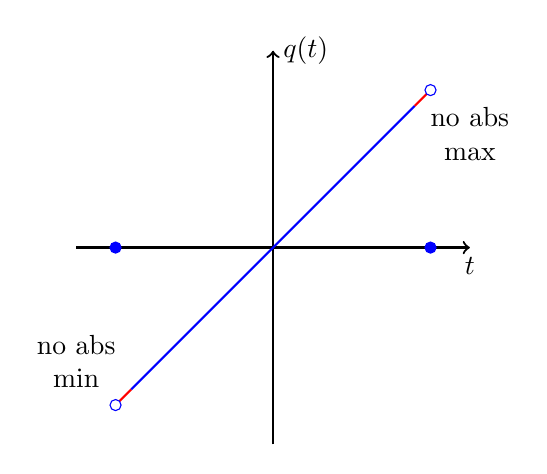
\begin{tikzpicture}
[
	closedpt/.style={circle,draw,fill,inner sep=0pt,minimum size=4pt},
	openpt/.style={circle,draw,inner sep=0pt,minimum size=4pt},
	scale=2
]

	% axes
	\draw[->,thick] (\xmin,0) -- (\xmax,0) node[below] {$t$};
	\draw[->,thick] (0,\ymin) -- (0,\ymax) node[right] {$q(t)$};

	% graph
	\draw[thick, red] (-1,-1) -- (-0.9,-0.9);
	\draw[thick, blue] (-0.9,-0.9) -- (0.9,0.9);
	\draw[thick, red] (0.9,0.9) -- (1,1);

	\node[blue,openpt,fill=white] at (-1,-1) {};
	\node[blue,openpt,fill=white] at (1,1) {};
	\node[blue,closedpt] at (-1,0) {};
	\node[blue,closedpt] at (1,0) {};

	\node[below,yshift=-0.1cm,xshift=0.5cm,align=center]
	  at (1,1) {no abs \\ max};
  	\node[above,yshift=0.1cm,xshift=-0.5cm,align=center]
	  at (-1,-1) {no abs \\ min};

\end{tikzpicture}
